\documentclass[review]{elsarticle}

\usepackage{lineno,hyperref}
\usepackage{pdflscape}
\modulolinenumbers[5]

\journal{Geochemica and Cosmochemica Acta}

%%%%%%%%%%%%%%%%%%%%%%%
%% Elsevier bibliography styles
%%%%%%%%%%%%%%%%%%%%%%%
%% To change the style, put a % in front of the second line of the current style and
%% remove the % from the second line of the style you would like to use.
%%%%%%%%%%%%%%%%%%%%%%%

%% Numbered
%\bibliographystyle{model1-num-names}

%% Numbered without titles
%\bibliographystyle{model1a-num-names}

%% Harvard
\bibliographystyle{model2-names.bst}\biboptions{authoryear}

%% Vancouver numbered
%\usepackage{numcompress}\bibliographystyle{model3-num-names}

%% Vancouver name/year
%\usepackage{numcompress}\bibliographystyle{model4-names}\biboptions{authoryear}

%% APA style
%\bibliographystyle{model5-names}\biboptions{authoryear}

%% AMA style
%\usepackage{numcompress}\bibliographystyle{model6-num-names}

%% `Elsevier LaTeX' style
%\bibliographystyle{elsarticle-num}
%%%%%%%%%%%%%%%%%%%%%%%

\begin{document}

\begin{frontmatter}

\title{Modelling excess properties of mineral and melt solutions over large P-T ranges: implications for phase relations and seismic velocities in the mantle}
%\tnotetext[mytitlenote]{Fully documented templates are available in the elsarticle package on \href{http://www.ctan.org/tex-archive/macros/latex/contrib/elsarticle}{CTAN}.}

%% Group authors per affiliation:
\author{R. Myhill}
\address{Bayerisches Geoinstitut, Universit\"{a}t Bayreuth, Universit\"{a}tsstrasse 30, 95447 Bayreuth, Germany}
\cortext[mycorrespondingauthor]{Corresponding author: R. Myhill}
\ead{myhill.bob@gmail.com}

\begin{abstract}
  Thermodynamic models of solid and liquid solutions in the Earth Sciences are increasingly used to calculate phase relations and seismic properties over large pressure and temperature ranges. Calculations often span over 1000 K and 5 GPa in studies of exhumation processes and metamorphism in subduction zones. Research into mantle phase relations and differentiation of the early Earth frequently involves calculations over 3000 K and 100 GPa. Despite spanning such huge ranges, a common approximation is that excess thermodynamic derivatives within solid solutions (entropy and volume) are pressure-temperature invariant. If these excesses are large, the approximation can result in large errors in gibbs free energy at high pressure and temperature, and errors in seismic velocities even within the range of calibration conditions. 

  In this paper, we present a solution to this problem by extending the subregular Margules mixing model using intermediate compounds to define the thermodynamic properties of solid solutions. Mathematical derivations are provided for excess properties ($H^{ex}$, $S^{ex}$, $V^{ex}$) and their pressure and temperature derivatives ($K_T^{ex}$, $\alpha^{ex}$, $Cp^{ex}$ etc.). We provide examples of pyroxene, garnet and melt solutions, showing that inclusion of a variable excess volume is vital to simulate observed phase relations and seismic velocities. Heuristics are suggested for intermediate compounds where individual thermodynamic properties are poorly constrained.


\end{abstract}

\begin{keyword}
high pressure \sep excess properties
\end{keyword}

\end{frontmatter}

\linenumbers

\section{Introduction}

Solution models are a vital part of estimating phase relations in the Earth. Typically, some functional form (often quadratic, cubic) is used to describe excess non-configurational energies between endmembers. Where necessary, the parameters describing the properties of the solid solution are allowed to vary as a function of pressure and temperature. 
\begin{equation}
  W_{ij} = W_{ij}^H + W_{ij}^VP + W_{ij}^ST
  \label{eqn:trad_form}
\end{equation}

Models described in this way have been extremely successful in describing the properties of solid solutions up to pressures of a few GPa. Increasingly, such models are being used over larger and larger pressure ranges. For example, garnet models are now being used to estimate phase relations in the mantle transition zone, and models of metallic alloys and melts are being used to study the composition and evolution of the Earth's core. Another development is the increasing use of solution models to estimate seismic velocities in the mantle and core. These two developments present a problem for the traditional approach described in Equation \ref{eqn:trad_form}, because they are both strongly dependent on the change in excess volume with pressure, a variable which is generally not zero.

We introduce here a simple adaptation of mixing models, which use intermediate compounds to describe the excess properties of the solid solution as a function of pressure and temperature. With this added flexibility comes a large increase in the number of free parameters, so we also provide useful heuristics for the cases where individual parameters are unknown.

The new form of the model is illustrated with the use of three implementations for pyroxene, garnet and Fe-FeO melt. We show that for these cases: a constant excess volume based on room pressure data is a bad approximation beyond a few GPa pressure, and major errors in seismic velocities and phase relations result from not incorporating reasonable decays in excess volume. The models in this study are all implemented in the open software \emph{burnman}, a mineral physics toolkit written in python. The software, first described in \cite{CHRU2014}, was originally designed for seismic velocity calculations. It has since been augmented with thermodynamics functionality, including a range of different models for solid solutions.

\section{The Extended Subregular Margules (ESM) model}
The subregular Margules mixing model within a binary system $A$-$B$ approximates excess Gibbs free energies at any given pressure and temperature as a cubic function of composition \citep{HW1989}:
\begin{equation}
  \mathcal{G}^{xs} = X_B (1-X_B) \left(W_{AB} X_B + W_{BA} (1-X_B) \right)
  \label{eqn:subreg}
\end{equation}

In the special case that $W_{AB} = W_{BA}$, the function is a quadratic. We can define the Gibbs interaction parameter in terms of the Gibbs free energy of a 50:50 intermediate compound ($AB$) and the endmembers $A$ and $B$:

\begin{equation}
  W^{\mathcal{G}}_{AB} = 4(\mathcal{G}_{AB} + T\mathcal{S}^{\textrm{conf}}_{AB}) - 2(\mathcal{G}_A + \mathcal{G}_B)
\end{equation}
\noindent where $\mathcal{S}^{\textrm{conf}}_{AB}$ is the configurational entropy of the intermediate compound. In the more general case that $W_{AB} \neq W_{BA}$, Equation \ref{eqn:subreg} can be thought of as two symmetric interaction parameters with contributions that depend on the composition. Two intermediate compounds ($AB$ and $BA$) are then required to describe the properties of the solution (Figure \ref{fig:schematic}).

\begin{figure}[ht!]
  \centering
  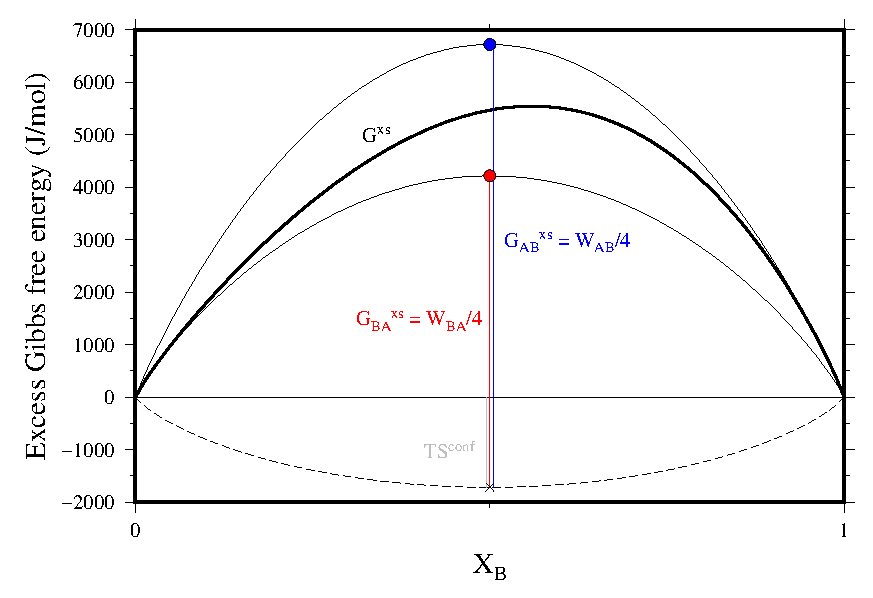
\includegraphics[width=0.8\textwidth]{figures/schematic}
  \caption{Schematic illustration of a binary subregular solution model.}
  \label{fig:schematic}
\end{figure}


Expanding the subregular solution model beyond a binary system, the excess nonconfigurational Gibbs free energy is \citep{HW1989} 
\begin{equation}
  \mathcal{G}^{xs} = \sum_{i=1}^n \sum_{j>1}^n X_i X_j \left ( W_{ij} X_j + W_{ji} X_i + 0.5 (W_{ij} + W_{ji}) \sum_k^n (1-\delta_{ik})(1-\delta_{jk}) X_k \right)
  \label{xs}
\end{equation}

Each of the individual $W_{ij}$ terms in Equation \ref{xs} can be determined via the properties of an intermediate compound, just as described in the binary $A$-$B$ system (Equation \ref{eqn:subreg}). The properties of the solid solution with composition ${X_i}$ are then defined as follows:

\begin{eqnarray}
\mathcal{G} = \sum_i X_i \mathcal{G}_i + \mathcal{G}^{xs} \\
\mathcal{H} = \sum_i X_i \mathcal{H}_i + \mathcal{H}^{xs} \\
\mathcal{S} = \sum_i X_i \mathcal{S}_i + \mathcal{S}^{xs} \\
\mathcal{V} = \sum_i X_i \mathcal{V}_i + \mathcal{V}^{xs} \\
C_P = \sum_i X_i C_P  + T \left( \frac{\partial \mathcal{S}}{\partial T} \right)_P^{xs} \\
\alpha = \frac{1}{\mathcal{V}} \left ( \sum_i X_i \alpha_i \mathcal{V}_i + \left( \frac{\partial \mathcal{V}}{\partial T} \right)_P^{xs} \right) \label{alpha} \\
K_T = \frac{\mathcal{V}}{\sum_i \frac{X_i \mathcal{V}_i }{K_{Ti}} - \left( \frac{\partial \mathcal{V}}{\partial P} \right)_T^{xs} } \label{K_T} \\
C_V = C_P - \mathcal{V} T \alpha^2 K_T \\
K_S = K_T \frac{C_P}{C_V} \\
\gamma = \frac{\alpha K_T \mathcal{V}}{C_V}   
\end{eqnarray}

With the exception of the enthalpy excess, excess terms ($\mathcal{S}^{xs}$, $\mathcal{V}^{xs}$ etc) are derived in the same way as the excess Gibbs free energy (Equation \ref{xs}), with interaction terms defined as follows:

\begin{eqnarray}
  W^{\mathcal{S}}_{ij} = 4 (\mathcal{S}_{ij} - \mathcal{S}^{\textrm{conf}}_{ij}) - 2(\mathcal{S}_i + \mathcal{S}_j) \\
  W^{\mathcal{V}}_{ij} = 4 \mathcal{V}_{ij} - 2(\mathcal{V}_i + \mathcal{V}_j) \\
  W^{\partial\mathcal{V}/\partial P}_{ij} = -4 \mathcal{V}_{ij}/K_{T{ij}} + 2(\mathcal{V}_{i}/K_{T{i}} + \mathcal{V}_{j}/K_{T{j}}) \\
  W^{\partial\mathcal{V}/\partial T}_{ij} = 4 \alpha_{ij} \mathcal{V}_{ij} - 2(\alpha_{i} \mathcal{V}_i + \alpha_{j} \mathcal{V}_j) \\
  W^{\partial\mathcal{S}/\partial T}_{ij} = \frac{4 C_{P{ij}} - 2(C_{P{i}} + C_{P{j}})}{T} 
\end{eqnarray}

Finally, excess enthalpy is defined as
\begin{equation}
 \mathcal{H}^{xs} = \mathcal{G}^{xs} + T\mathcal{S}^{xs}
\end{equation}

\subsection{Heuristics}
It is often the case that endmembers are particularly well studied, while the properties of the solid solution are constrained only by enthalpies of solution and volumes at room temperature and pressure. The remaining properties of the intermediate compounds must be estimated by the user. In this study, we suggest that the following heuristics be used:
\begin{eqnarray}
  \mathcal{S}_{ij} = 0.5(\mathcal{S}_i + \mathcal{S}_j) + \mathcal{S}^{\textrm{conf}}_{ij} \\
  C_{P{ij}} = 0.5(C_{P{i}} + C_{P{j}}) \\
  \alpha_{ij} = 0.5 \mathcal{V} \left(\frac{\alpha_i}{\mathcal{V}_i} + \frac{\alpha_j}{\mathcal{V}_j}\right)\\
  K'_{T} = -\frac{\partial}{\partial P} \left (\mathcal{V}\left( \frac{\partial P}{\partial \mathcal{V}} \right)_T \right) \sim \mathcal{V} \left(\sum_i \frac{X_i \mathcal{V}_i}{K'_{Ti} + 1} \right)^{-1} - 1
\end{eqnarray}

If excess volumes are zero, it is likely that they will remain zero as temperatures and pressures increase. In this case, the bulk modulus is given by Equation \ref{K_T}, with the differential term equal to zero. In contrast, non-zero excess volumes are unlikely to remain constant with pressure and temperature. Mixing of elements with different ionic radii and field strengths result in lattice distortions, and a series of weaker or stronger bonds. It is reasonable to assume that a positive volume excess results in longer bonds which are, on average, more compressible, and that a negative volume excess results in reduced compressibility. In this case, a positive volume excess results in a negative excess bulk modulus. We suggest that, in the absence of other data a useful heuristic is the suggestion that $\left( \frac{\partial \mathcal{V}}{\partial P} \right)_T^{xs} \rightarrow 0$ as $P \rightarrow \infty$.

A useful way to view the change in bulk modulus across a solid solution is to compare the excess bulk modulus to that implied by the $K_TV =$ \emph{constant} rule of thumb proposed by \cite{AA1970} to estimate the compressibility of endmembers based on their molar volumes. The heuristic we propose in this study predicts a larger excess term than that suggested by the rule of thumb, which we describe using a factor $\xi$:

\begin{equation}
  K_{T} \sim 0.5(K_{Ti} + K_{Tj}) + \xi \left(\frac{K_{Ti}\mathcal{V}_{j} + K_{Tj}\mathcal{V}_{j}}{\mathcal{V}_{i} + \mathcal{V}_{j}} - 0.5(K_{Ti} + K_{Tj})\right)
  \label{K_T_heuristic}
\end{equation}
\noindent Typically, a value of $\sim$6 provides a useful estimate of $\xi$.

Now that we have described the new model, we turn to a few geologically relevant examples.

\section{Examples}
\subsection{Pyroxene}
Our first example is that of jadeite-aegirine pyroxene, an almost ideal solid solution (from a volumetric perspective). We use this model to illustrate that even when excess volumes are extremely small, excess bulk moduli are resolvable. The experimental data is that of \cite{NBLBT2006}, and the equation of state used is the Modified Tait \citep{HP2011}. The fit to the volume data is shown in Figure \ref{fig:PV_jadeite_aegirine}.

\begin{figure}[ht!]
  \centering
  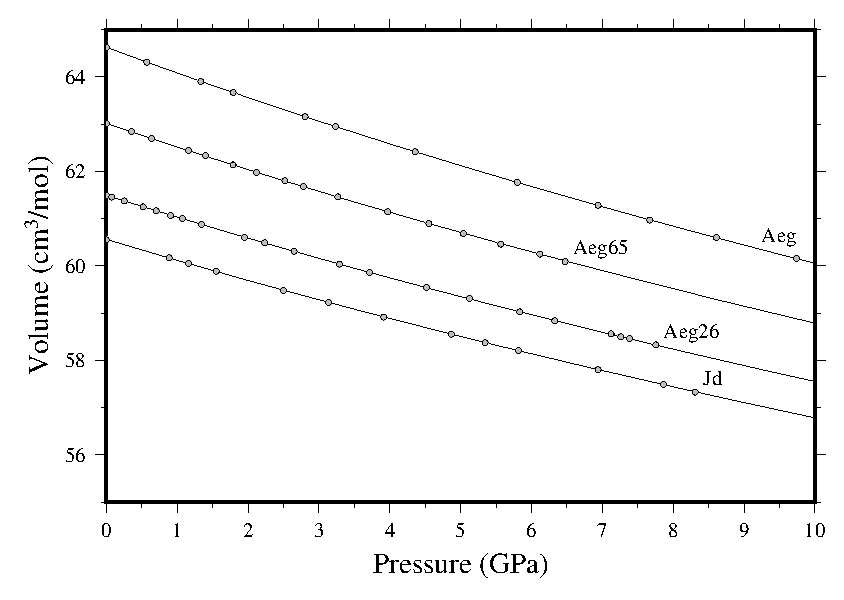
\includegraphics[width=0.8\textwidth]{figures/jadeite_aegirine_P_V}
  \caption{Pressure-volume data in the binary system Jadeite-Aegirine \citep{NBLBT2006}, with the model proposed in this study.}
  \label{fig:PV_jadeite_aegirine}
\end{figure}

\begin{table}[ht!]
\centering
\caption{Jadeite-Aegirine mixing parameters to fit the room temperature data of \cite{NBLBT2006}. The $K'_0$ for the intermediate compound is fixed to the value given by the heuristic proposed in the text. $K''_0 = -K'_0/K_0$.}
\label{tab:jd_aeg}
\begin{tabular}{lllll}
                   & jadeite              & aegirine             & jd$_{50}$ae$_{50}$             & ae$_{50}$jd$_{50}$             \\
$V_0$ (cm$^3$/mol) & 60.5640 $\pm$ 0.0001 & 64.6261 $\pm$ 0.0004 & 62.3641 $\pm$ 0.0005 & 62.4522 $\pm$ 0.0005 \\
$K_0$ (GPa)        & 133.5 $\pm$ 0.2      & 116.0 $\pm$ 0.2      & 124.8 $\pm$ 0.5      & 126.7 $\pm$ 0.4      \\
$K'_0$             & 4.6 [fixed]                 & 4.4 [fixed]                 & 4.4785 [heuristic]              & 4.4785  [fixed]           
\end{tabular}
\end{table}

Using the derived properties of the solid solution, we can fit the excess volume as a function of pressure (Figure \ref{fig:excess_volume_jadeite_aegirine}). The decay of excess volume as a function of pressure is in excellent agreement with the prediction that excess volumes decay to zero at extreme pressures. For the 50:50 intermediate, the Equation \ref{K_T_heuristic} is satisfied when $\xi \sim$ 10.

\begin{figure}[ht!]
  \centering
  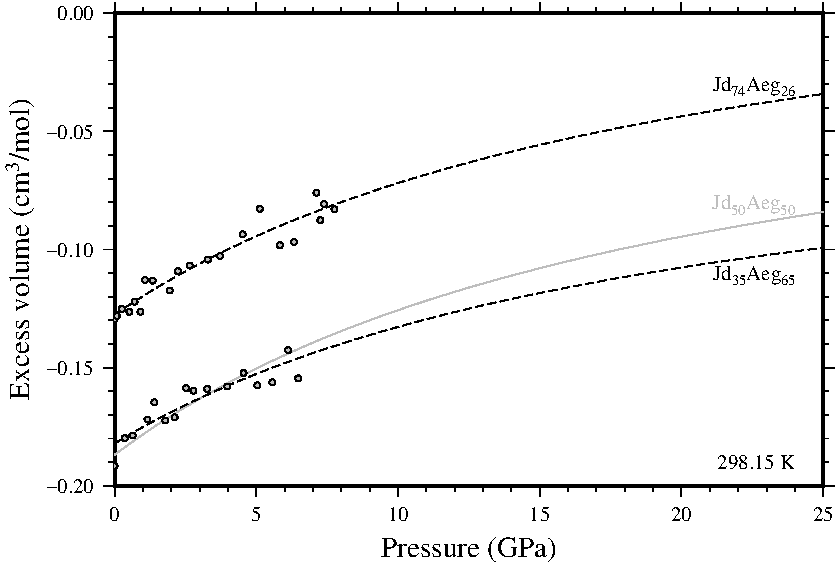
\includegraphics[width=0.8\textwidth]{figures/jadeite_aegirine_Vex}
  \caption{Excess volume for Jd-Aeg pyroxenes calculated from our model.}
  \label{fig:excess_volume_jadeite_aegirine}
\end{figure}

\clearpage
\subsection{Garnet}
Our second example is the pyrope-grossular join, which is well-known to have significant non-ideality and volumes of mixing \citep{NCK1977, BG1997, GCT1996}. Recently, it has been suggested that the excess volumes of mixing are $\sim$1 cm$^3$/mol, 2--3 times larger than previously suggested, and associated with very large negative excess bulk moduli \citep{DCW2015}. If this were true, it would have significant implications for phase relations and seismic velocities in the mantle.

Here, we create four models to describe the room temperature equations of state for the pyrope-grossular system. Two models are presented for the data of \citep{DCW2015}, to describe the reported behaviour close to the center and at the edges of the solid solution. The third model is the constant volume subregular Margules model of \cite{GCT1996}. A fourth model has the same excess volume as \cite{GCT1996}, but a negative excess bulk modulus which allows the excess volume to decay to zero at high pressures. The standard state bulk moduli are shown in Figure \ref{fig:K_T_pyrope_grossular}.


\begin{table}[ht!]
\centering
\caption{Pyrope-Grossular mixing parameters to fit the P-V-T data of \cite{DCW2015}. The $K'_0$ for the ordered intermediate compound is fixed to the value given by the heuristic proposed in the text. The extreme $K_0$ and $K'_0$ for the disordered intermediate compound are required to avoid negative volume excesses at high pressure. $K''_0 = -aK'_0/K_0$, where $a=1$ and $a=52$ for the ordered and disordered compounds respectively.}
\label{tab:py_gr}
\begin{tabular}{lllll}
                   & pyrope              & grossular             & py$_{50}$gr$_{50}$ (ord)  & py$_{50}$gr$_{50}$  (disord)   \\
$V_0$ (cm$^3$/mol) & 113.14 $\pm$ 0.02 &  125.18 $\pm$ 0.03      & 120.13 $\pm$ 0.03  & 119.63 $\pm$ 0.06 \\
$K_0$ (GPa)        & 168 $\pm$ 2       &  173 $\pm$ 2            & 159 $\pm$ 3   &    127 [see caption]  \\
$K'_0$             & 4.4 [fixed]              &  5.5 [fixed]     & 4.975 [heuristic]  &  22 [see caption] \\
$\alpha_0$ (10$^{-5}$/K)   &  2.58 $\pm$ 0.06   & 2.15 $\pm$ 0.05 & 2.12 $\pm$ 0.07  & 1.88 $\pm$ 0.16
\end{tabular}
\end{table}


\begin{figure}[ht!]
  \centering
  %\includegraphics[width=0.8\textwidth]{figures/pyrope_grossular_K_T}
  \caption{Bulk moduli in the binary system Pyrope-Grossular \citep{DCW2015}, with the models proposed in this study.}
  \label{fig:K_T_pyrope_grossular}
\end{figure}

XXXX Discussion


These models are now used to illustrate the effect of decaying excess volumes on seismic wave velocities. P-wave, S-wave and bulk sound velocities are functions of isentropic bulk and shear moduli and density:
\begin{eqnarray}
V_P = \sqrt \frac{K_S + \frac{4}{3} G }{\rho} \\
V_S = \sqrt \frac{G}{\rho} \\
V_\Phi = \sqrt \frac{K_S}{\rho}
\end{eqnarray}
Thermodynamic solution models say nothing about shear moduli, so we restrict our discussion to the bulk sound velocity. Figure \ref{fig:bulk_sound_garnet} shows the bulk sound velocity at ambient temperature for the four solid solution models in the text. XXXX Discussion %reduction of bulk sound velocities for the ``ordered'' endmember is $\sim$5\%, comparable to the variation of seismic wavespeeds in the mantle at a given depth. Also noteworthy is the difference in pressure dependence of the bulk sound velocities between the two models presented in this study. To avoid negative excess volumes in the ``disordered'' endmember, it was necessary to choose a very large $K'_0$. As a result, the excess volumes decay very rapidly, and the seismic wavespeeds at low pressures are extremely low. It is currently unclear what the volume behaviour of pyrope-grossular garnets is at high temperatures and pressures of 10--25 GPa, but the implication of our work is that using constant positive (or negative) excess volumes can significantly overestimate (underestimate) seismic velocities and/or underestimate (overestimate) the stability of intermediate compounds.

\begin{figure}[ht!]
  \centering
  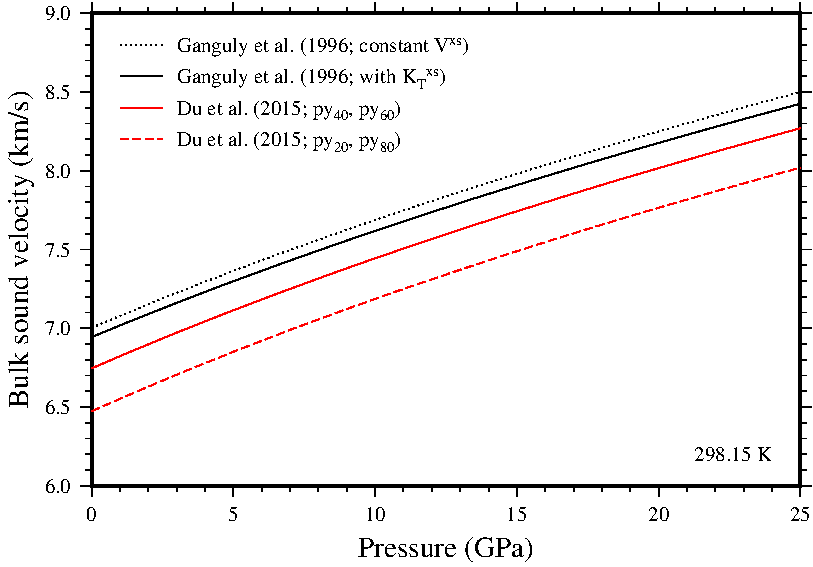
\includegraphics[width=0.8\textwidth]{figures/pyrope_grossular_bulk_sound_velocities}
  \caption{Bulk sound velocities of Py$_{50}$Gr$_{50}$ at room temperature according to the model of \citep{GCT1996}, a fixed excess volume based on room pressure data \citep{DCW2015} and the two full subregular models incorporating excess bulk moduli introduced in the present study.}
  \label{fig:bulk_sound_garnet}
\end{figure}



\clearpage
\subsection{Fe-FeO melt}

Our final example is that of Fe-FeO melt. As oxygen may be one of the more abundant light elements in the core, understanding the thermodynamics of this liquid solution is an important part of understanding mantle-core differentiation and interaction over billions of years. At pressures $<$25 GPa, the Fe-FeO solution exhibits signficant non-ideality, with a large miscibility gap between ionic and metallic Fe-O liquids \citep{KS1995,TOT2007,Frostetal2010}. As pressure increases, this miscibility gap disappears, indicating a negative excess volume of mixing (Figure \ref{fig:Fe_O_solvus}). To explain the increase in eutectic temperature with pressure, \cite{Kom2014} suggest that mixing becomes essentially ideal at $>$100 GPa. 

\begin{figure}[ht!]
  \centering
  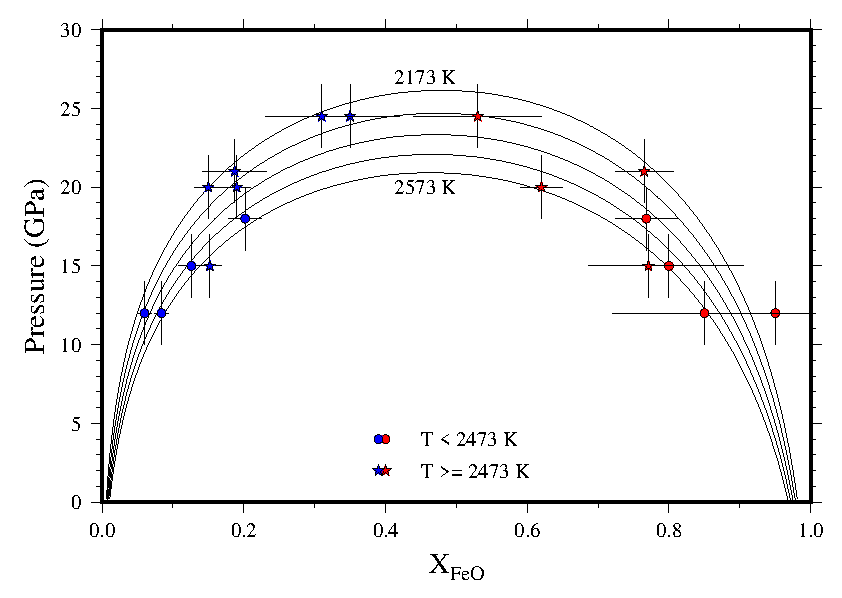
\includegraphics[width=0.8\textwidth]{figures/Fe_FeO_solvus}
  \caption{Fe-O solvus}
  \label{fig:Fe_O_solvus}
\end{figure}


To model processes of mantle differentiation and core formation, it would be extremely useful to have a single model describing the properties of melts over relevant pressure and temperature ranges. Clearly a high pressure ideal model cannot be reconciled with a low pressure model with large excess volumes of mixing without incorporating excess bulk moduli and thermal expansivities. Below $\sim$25 GPa, the properties of the liquid can be estimated using the compositions of coexisting metallic and ionic liquid \citep{TOT2007,Frostetal2010}. The chemical potentials of Fe and FeO are equal in the ionic and metallic liquids, providing the two constraints necessary to estimate Margules parameters at each pressure and temperature (Figure \ref{fig:Fe_O_interaction}).

\begin{figure}[ht!]
  \centering
  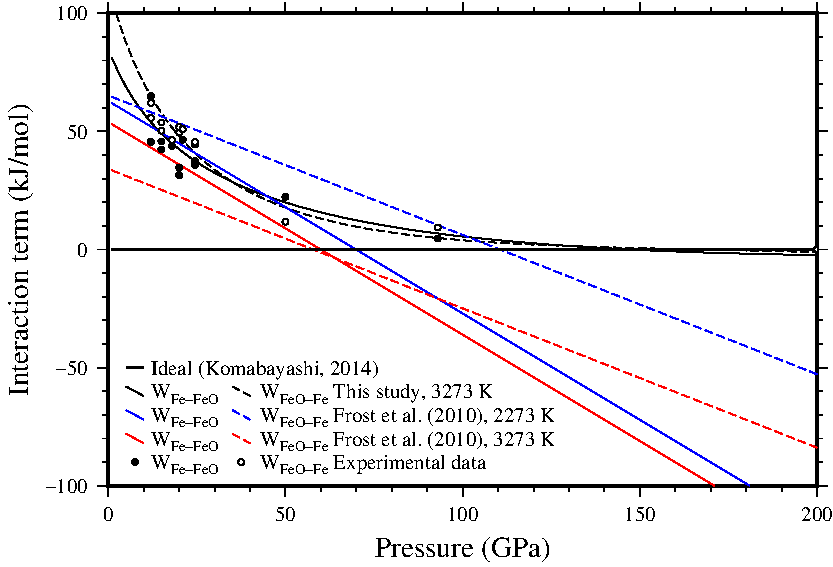
\includegraphics[width=0.8\textwidth]{figures/Fe_FeO_interaction_terms}
  \caption{Interaction terms in Fe-FeO melt as a function of pressure.}
  \label{fig:Fe_O_interaction}
\end{figure}

At $>$25 GPa, the pressure, temperature and compositions of eutectic liquid at high pressure \citep{SHCPW2008} provide further constraints, providing we know the relative gibbs free energies of liquid and solid Fe and FeO. Here, we fit the thermodynamic properties of the FCC and HCP iron endmembers and of B1 FeO to published P-V-T data and phase boundaries. The liquid endmembers are fit with available room pressure data, and the effect of pressure is estimated using constraints on the melting curves from \cite{ADMLM2013}, \cite{SHCPW2008} and \cite{OTHOH2011}. The uncertainties on composition and temperature of the eutectic are rather large, so these data are supplemented by the requirement that excess volumes become zero at very high pressure. The parameters used to create the fits in Figures \ref{fig:Fe_O_interaction} and \ref{fig:Fe_O_melting} are given in Table \ref{tab:Fe_FeO}. In this work, we fix excess entropy and thermal expansion to zero. The majority of the $<$25 GPa data was collected within a $\sim$200 K temperature range, and is associated with similar temperature uncertainties, which introduces very large uncertainties in excess entropies. Add to that the possibility of phase separation during quench and the large uncertainty in coexisting ionic/metallic melt compositions, there is no clear evidence for the large temperature dependence proposed by \cite{Frostetal2010}, although they do slightly improve the fit to the data (mostly by increasing the pressure at which the solvus closes at high temperature).

\begin{figure}[ht!]
  \centering
  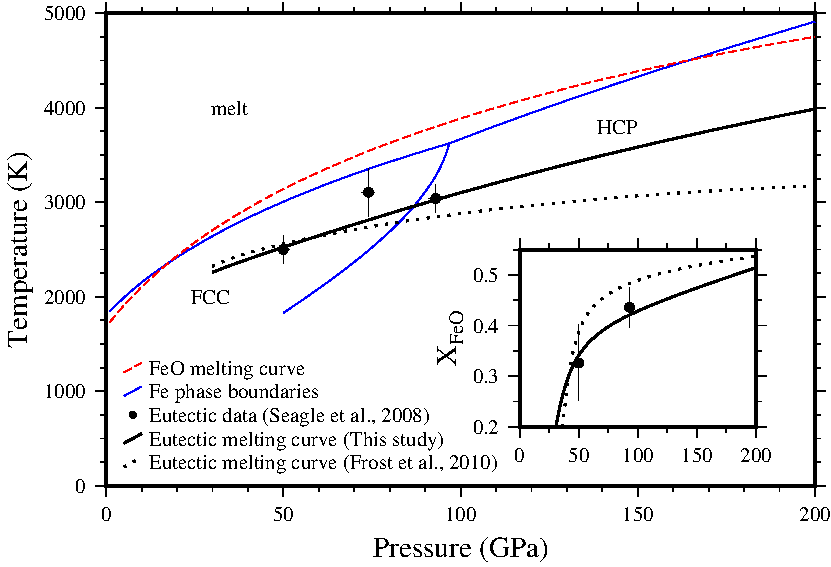
\includegraphics[width=0.8\textwidth]{figures/Fe_FeO_T_X_eutectic}
  \caption{Melting temperature in the Fe-O system as a function of pressure. Inset: eutectic composition in the Fe-O system.}
  \label{fig:Fe_O_melting}
\end{figure}

\begin{table}[ht!]
\centering
\caption{Excess Fe-FeO mixing parameters to fit the data in Figures \ref{fig:Fe_O_interaction} and \ref{fig:Fe_O_melting} at a reference temperature of 1809 K and pressure of 50 GPa.}
\label{tab:Fe_FeO}
\begin{tabular}{lll}
  Property        & Fe$_{50}$FeO$_{50}$  & FeO$_{50}$Fe$_{50}$ \\
  $H^{xs}$ (J/mol) &  5000 $\pm$ 400 & 4400 $\pm$ 400  \\
  $S^{xs}$ (J/K/mol)  & 0 [fixed] & 0 [fixed] \\
  $V^{xs}$ (cm$^3$/mol)   & -0.117 $\pm$ 0.009 &  -0.136 $\pm$ 0.009 \\
  $K^{xs}$  (GPa)  & 28 $\pm$ 5 & 45 $\pm$ 5  \\
  $K'^{xs}$   & -0.07 $\pm$ 0.12 & -0.37 $\pm$ 0.12  \\
  $a^{xs}$   & 0 [fixed] & 0 [fixed]  
\end{tabular}
\end{table}

\clearpage
\section{Discussion}

The use of intermediate compounds to describe excess properties is an extremely simple but powerful concept that lends a great deal of flexibility to models without necessarily increasing the number of parameters which need to be fit to the available experimental data. We note that the equations derived here are all quite general, and therefore easily applicable to a wide range of different equations of state.

The heuristics suggested here place constraints on seismic properties which are significantly more strict than typical uncertainties on bulk moduli derived from ultrasonic interferometry, Brillouin scattering or static compression. For example, along the pyrope-majorite join, excess volumes are small (0.1 cm$^3$/mol) \citep{HSSR1997}. With the assumption that excess volumes decrease to zero with increasing pressure, the excess bulk modulus is constrained to be $\sim$-0.6 GPa. In comparison, the range in bulk modulus estimates anywhere along the pyrope-majorite join is about 10 GPa \citep[see, for example][]{HDWB2010}. So far, high pressure elasticity studies have mostly been focussed on binary joins with small excess volumes at ambient pressure \citep{FXMLX2015, HC2014}. That they should small excess bulk moduli is in good agreement with the heuristics proposed here, but a far more rigorous test would be to investigate systems with large volume excesses.

It is envisaged that the model formulation proposed in this study will be very useful in modelling silicate and metallic melts, where excess volumes are large at low pressure. Even in the MgO-SiO$_2$ system, excess entropies and volumes are strongly dependent on temperature and pressure \citep{DKS2013}.


\section{Acknowledgments}
RM is funded by the Advanced ERC Grant awarded to the ``ACCRETE'' project.
\clearpage
\section*{References}

\bibliography{references_xs}

\end{document}
